\documentclass{report}
\usepackage[utf8]{inputenc}
\usepackage{amsmath}
\usepackage{graphicx,float}
\usepackage{caption}
\usepackage{subcaption}
\usepackage{gensymb}
\usepackage[margin=1.25in]{geometry}

\title{Sound Field Control with a Coaxial, Cardioid, Axisymmetric Loudspeaker}
\author{Alex Booth, supervised by Jonathan Hargreaves\\ a.booth9@edu.salford.ac.uk}

\begin{document}

\maketitle

\chapter*{Declaration}

\chapter*{Abstract}
    \textit{}

\chapter*{Dedication}



\chapter*{Acknowledgements}

\tableofcontents
\newpage

\chapter{Introduction}
    OPENING
        The directionality of a loudspeaker can be a definitive tool of active sound field control.
    BACKGROUND

    RESEARCH PROBLEM

    Axisymmetric cardioid loudspeaker (ACL for the rest of this paper.)

    AIMS

    SIGNIFICANCE

    LIMITATIONS

    STRUCTURE



\chapter{Literature Review}
    AUTHOR'S PROBLEM
    KEY CONCEPTS IN SOURCE
    KEY THEORIES
    DO THEY INNOVATE OR REFINE?
    CONCLUSIONS?
    HOW DOES IT RELATE TO OTHER LITERATURE?
    STRENGTHS?
    WEAKNESSES?

    SOUND FIELD CONTROL:




    DIRECTIONAL LOUDSPEAKERS:

    Harry Olson's `Gradient Loudspeakers'~\cite{olson1973gradient} forms the theoretical foundation of controlling the directionality of emitted sound with multiple loudspeaker drivers.
    The key concept Olson introduces is the `gradient loudspeaker', which are organized into orders.
    Zero-order gradient loudspeakers utilize a single driver within a sealed cabinet to give a theoretical monopole directionality, much like an omnidirectional microphone.
    Higher orders introduce directionality; a first-order unidirectional loudspeaker constructed with a spaced and delayed pair of zero-order gradient speakers operating 180\degree\@ out of phase gives a cardioid response.
    Olson gives the radiated pressure of this unidirectional gradient loudspeaker, shown in Eq.\ref{olsonFirstOrderPressure}.
    \begin{equation}
        p = 2CU_f\cos{kct}[\sin{\frac{kd}{4}+\frac{kD}{4}\cos{\theta}}]
        \label{olsonFirstOrderPressure}
    \end{equation}
    \begin{figure}[H]
        \centering
        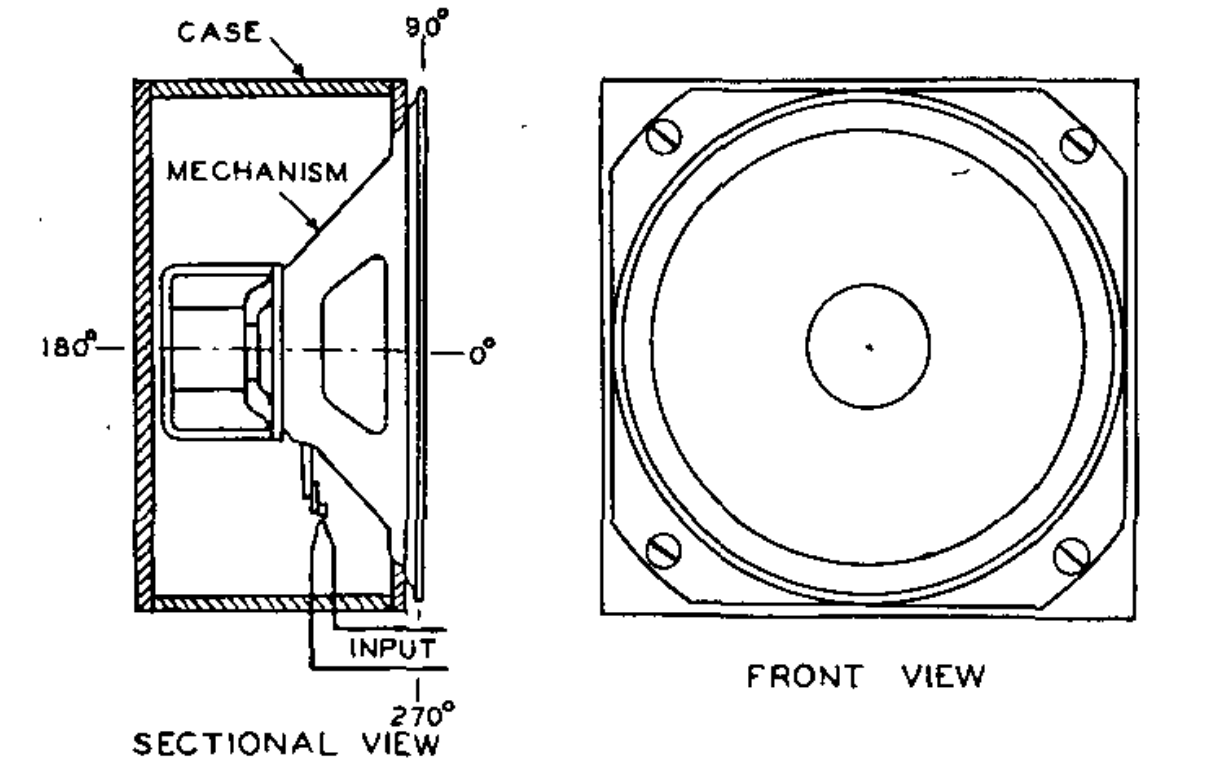
\includegraphics[scale=0.2]{figs/olsonFirstOrder.png}%
        \caption{Olson's first order unidirectional loudspeaker.}\cite{olson1973gradient}
        \label{olsonFirstOrderDiagram}
    \end{figure}
    Predating his work on gradient loudspeakers, Olson was an early descriptor of the beam narrowing effect of loudspeaker line arrays \cite{olson1957acoustical}.
    Line arrays would go on to be a principle tool of sound field control in the modern day.
    However, gradient loudspeakers are still, relative to line arrays, uncommon.
    Cardioid subwoofer systems used in live audio are common implementations of gradient loudspeaker designs.
    These subwoofers can be sold as gradient loudspeakers themselves, often with switchable directivity patterns; audio engineers will also arrange standard, omnidirectional subwoofers into configurations that introduce a phase delay sufficient to create a cardioid directivity pattern~\cite{curtis2022cardioidsubs}.

    COUPLED ENCLOSURE:

    The prototype ACL has each low-frequency driver mounted in a shared, acoustically coupled enclosure.
    Robustness and efficiency of an acoustically coupled two-source superdirective array, an ICSV22 paper by Jordan Cheer, elaborates on the benefits of such a shared enclosure \cite{cheer2015robustness}.
    Cheer acknowledges how a superdirective array of loudspeakers have `high sensitivity to uncertainties in the assumed response of the system', and that regularization of the powered signal driving units in an array can improve the `robustness to uncertainty'.
    However, he further notes that these measures may limit the directivity of a such a system; counterproductive to the designed purpose of a superdirective array.
    Robustness and efficiency thus sets out to investigate the robustness of acoustically coupled two-source superdirective loudspeaker, as opposed to the previously investigated non-interacting directional loudspeakers.
    Cheer finds, using a two-port model of loudspeaker behavior and derived simulations, that an uncoupled two-source array is `more significantly affected by response uncertainties than the coupled array', and thus the coupled array is more robust, avoiding the need for regularization.

    
    
    





    







\chapter{Theory}


\chapter{Methodology}
    \section{Transfer Function Measurement}
        SPEAKER WAS PUT IN THE ANECHOIC
        To build a numerical analysis of the directivity of the axisymmetric loudspeaker system's behavior as a whole over all frequencies, the frequency-domain transfer function of each driver must be measured across the entire X-Y AXIS MAYBE.
        In order to create a precise and accurate measurement free of interference and noise, the drivers were measured, mounted in the loudspeaker unit, in a fully anechoic chamber with a NTi reference-grade measurement mic.
        Ensuring the angle interval of each measurement was consistent, the loudspeaker was mounted to a Four Audio ELF robot arm which rotated the loudspeaker system about the X-Y AXIS MAYBE.
        Swept sine input signals were fed to each driver as the input excitation.
        The two low-frequency drivers were fed by a Samson SERVO-500 power amplifier, whilst the mid-high driver was fed by a University of Salford in-house made mono power amplifier, a 'Dial-a-Watt'.
        The output of the Dial-a-Watt was fed to a KEF-made cross-over, splitting the signal into mid and high frequency bands for the coaxial Uni-Q's mid and high drivers.
        The low frequency drivers had no cross-over filtering applied at this stage of the testing.
        The full signal flow of the transfer function measurement system is shown in Fig.\ref{signalFlow}.
        \begin{figure}[H]
            \centering
            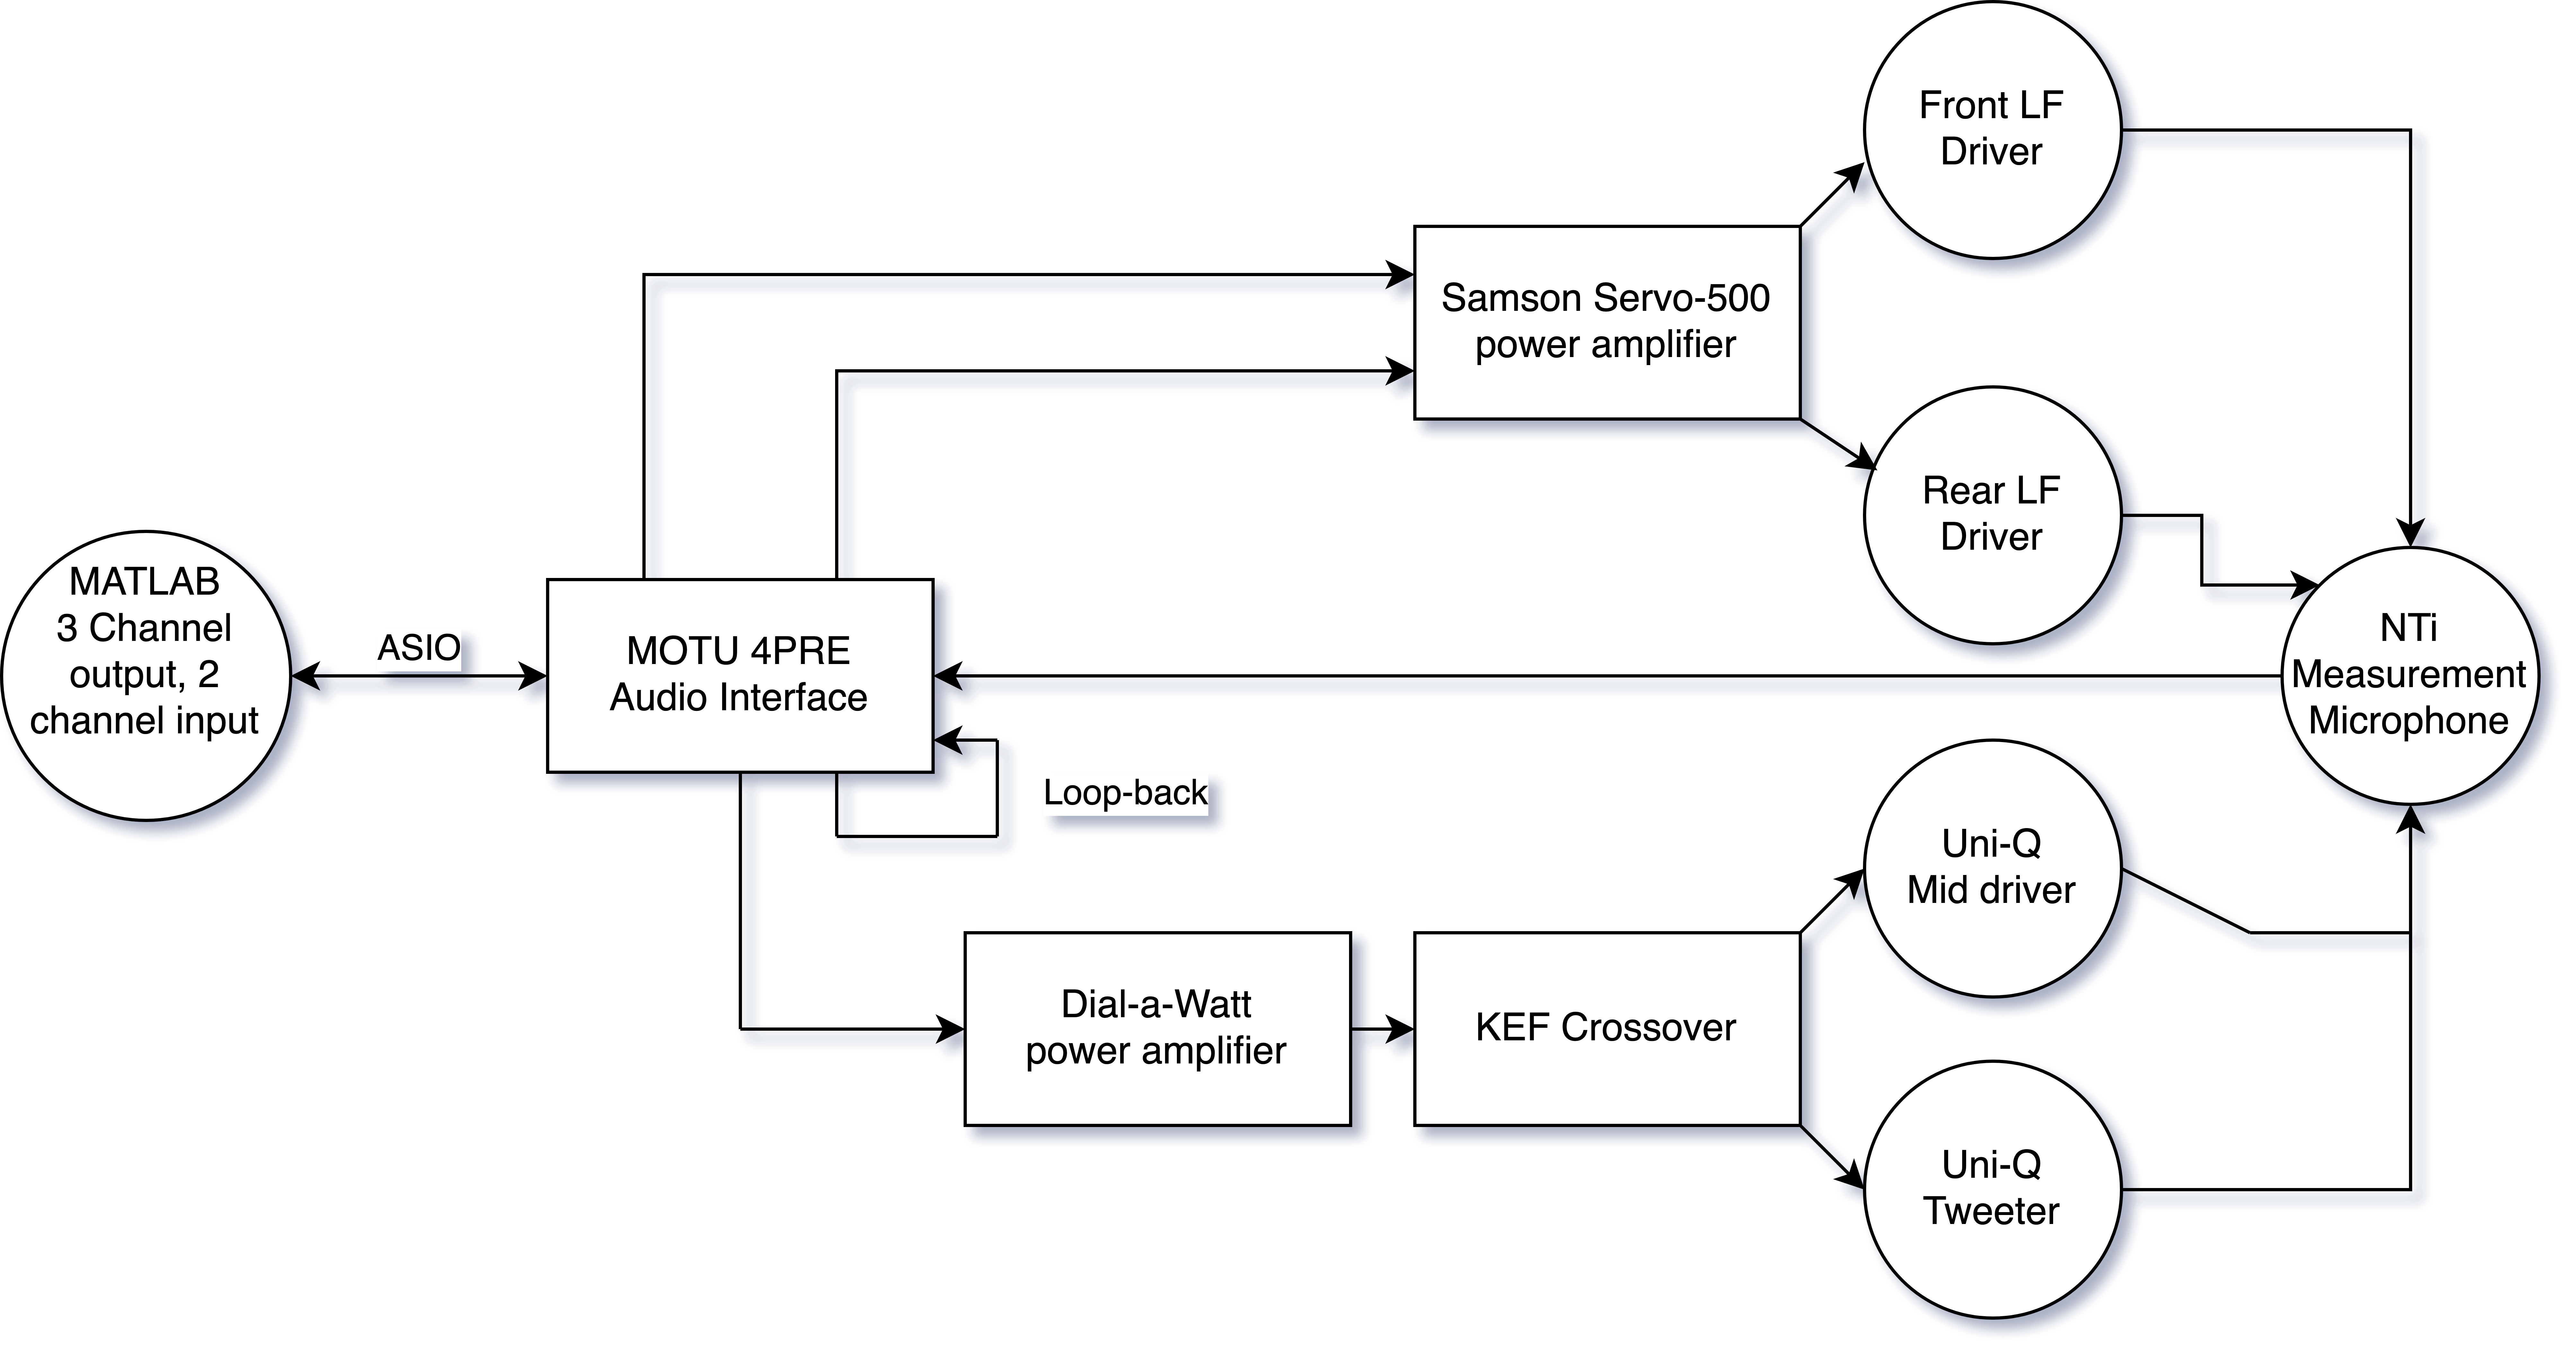
\includegraphics[scale=0.04]{figs/signalFlow.png}%
            \caption{Signal flow of driver transfer function measurement}
            \label{signalFlow}
        \end{figure}

        All audio output, robot arm movements and input recordings were automated through a MATLAB script.
        
        INTER M M700 POWER AMP
        DIAL-A-WATT at 2W
        KEF CROSSOVER FOR MID-HIGH
    

    

\chapter{Discussion and Conclusions}

\bibliographystyle{IEEEtran}
\bibliography{theBib.bib}

\end{document}


